\documentclass[aspectratio=169,11pt,xcolor=table]{beamer}
% Tema Berlin com cores e fonte padrão, sem cabeçalho de navegação e sem rodapé (visual limpo)
\usetheme{Berlin}
\setbeamertemplate{headline}{}
\setbeamertemplate{footline}{}
\usepackage[no-math]{fontspec}   % Latin Modern no texto; no-math deixa o beamer pôr a matemática sem serifa
\usepackage{amsmath}
\usepackage{amssymb}
\usepackage{icomma}   % vírgula decimal sem espaço dentro da matemática (ex.: $R^2 = 0,59$)
\usepackage{bm}
\usepackage{booktabs}
\usepackage{tabularx}
\usepackage{graphicx}
\usepackage{appendixnumberbeamer}

% Figuras e números vêm do código de entrega (entrega/) via gerar_numeros.R: nada é digitado à mão
\graphicspath{{../../entrega/resultados/eda/}{../../entrega/resultados/modelagem/}}

\definecolor{navy}{rgb}{0.2,0.2,0.7}   % mesmo azul da estrutura do tema padrão do beamer
\definecolor{ods}{HTML}{00689D}
\definecolor{destaque}{HTML}{C8343B}
\definecolor{verde}{HTML}{2E7D4F}
\definecolor{fundo}{HTML}{EAF1F7}
\setbeamercolor{alerted text}{fg=destaque}
\setbeamerfont{institute}{size=\footnotesize}
\setbeamerfont{date}{size=\footnotesize}
\setbeamertemplate{navigation symbols}{}
% Frame de encerramento: o gerar_briefings.R reconhece a opção "standout" pelo nome
\makeatletter\define@key{beamerframe}{standout}[true]{}\makeatother

\newcommand{\ok}{{\color{verde}\checkmark}}
\newcommand{\nao}{{\color{destaque}$\bm{\times}$}}
\newcommand{\fig}[1]{\includegraphics[width=\linewidth,height=0.66\textheight,keepaspectratio]{#1}}
% Fonte da figura ou tabela, no padrão "Fonte: ... Elaboração própria."
\newcommand{\fonte}[1]{\par\vspace{0.2em}{\tiny\color{black!60}Fonte: #1\par}}
\newcommand{\nMunBR}{5.570}
\newcommand{\nHomBR}{138.316}
\newcommand{\nTaxaBR}{22,7}
\newcommand{\nPopMin}{20}
\newcommand{\nMunEsc}{1.710}
\newcommand{\nPctPopEsc}{84}
\newcommand{\nZerosBR}{655}
\newcommand{\nTaxaMedia}{25,0}
\newcommand{\nTaxaMediana}{20,5}
\newcommand{\nAssimTaxa}{1,36}
\newcommand{\nAssimLn}{$-$0,49}
\newcommand{\nTaxaNE}{39,3}
\newcommand{\nTaxaSE}{13,2}
\newcommand{\nHomAno}{46.105}
\newcommand{\nTaxaMundo}{5,8}
\newcommand{\nRazaoMundo}{3,9}
\newcommand{\nTaxaNbr}{36,4}
\newcommand{\nTaxaNEbr}{36,9}
\newcommand{\nTaxaCObr}{22,2}
\newcommand{\nTaxaSEbr}{13,0}
\newcommand{\nTaxaSbr}{16,7}
\newcommand{\nMedAma}{30,1}
\newcommand{\nMedForaAma}{18,0}
\newcommand{\nMedFront}{18,4}
\newcommand{\nMedForaFront}{20,7}
\newcommand{\nCorMax}{0,56}
\newcommand{\nCorMaxVar}{\% preta/parda}
\newcommand{\nCorTrio}{0,92}
\newcommand{\nRendaDecilPico}{803}
\newcommand{\nPorteHomMenor}{1}
\newcommand{\nPorteOscMenor}{66}
\newcommand{\nPorteCorMenor}{0,26}
\newcommand{\nPorteCorMaior}{0,89}
\newcommand{\nPorteOscVinte}{23}
\newcommand{\nLambda}{0,18}
\newcommand{\nLambdaInf}{0,14}
\newcommand{\nLambdaSup}{0,22}
\newcommand{\nSWy}{0,92}
\newcommand{\nSWln}{0,98}
\newcommand{\nVIFrenda}{27}
\newcommand{\nRdoisA}{0,59}
\newcommand{\nRdoisAregiao}{0,51}
\newcommand{\nDWregiao}{1,71}
\newcommand{\nFuf}{15,9}
\newcommand{\nFblocoEd}{46,9}
\newcommand{\nRdoisAsemEd}{0,39}
\newcommand{\nRdoisAcomEd}{0,44}
\newcommand{\nFglobal}{62}
\newcommand{\nGlUm}{40}
\newcommand{\nGlDois}{1.669}
\newcommand{\nPico}{1.065}
\newcommand{\nBP}{110}
\newcommand{\nDW}{2,01}
\newcommand{\nDWp}{0,66}
\newcommand{\nSW}{0,98}
\newcommand{\nNout}{1}
\newcommand{\nSWp}{$<$0,001}
\newcommand{\nBPgl}{40}
\newcommand{\nBPp}{$<$0,001}
\newcommand{\nGlUF}{22}
\newcommand{\nPUF}{$<$0,001}
\newcommand{\nRdoisE}{0,60}
\newcommand{\nSigma}{0,521}
\newcommand{\nFglobalP}{$<$0,001}
\newcommand{\nVIFrendaFinal}{12,7}
\newcommand{\nVIFdemaisMax}{7,8}
\newcommand{\nNumUF}{26}
\newcommand{\nNumX}{12}
\newcommand{\nNumPar}{41}
\newcommand{\nCorQuadSem}{0,9995}
\newcommand{\nCorQuadCen}{$-$0,11}
\newcommand{\nBetaDois}{$-$0,548}
\newcommand{\nBetaDoisP}{$<$0,001}
\newcommand{\nOutNomes}{Nhamundá-AM}
\newcommand{\nIconeSW}{\ok}
\newcommand{\nTextoSW}{Normalidade razoável}
\newcommand{\nIconeOut}{\ok}
\newcommand{\nTextoOut}{1 outlier}
\newcommand{\nIconeDW}{\ok}
\newcommand{\nTextoDW}{Sem autocorrelação na ordem do código}
\newcommand{\nIconeBP}{\nao}
\newcommand{\nTextoBP}{Variância não constante}
\newcommand{\nNaoSig}{faixa de fronteira, \% homens 15–29, densidade}


\title{Fatores associados aos homicídios nos municípios brasileiros}
\subtitle{Uma análise de regressão linear múltipla \textbullet{} ODS 16, indicador 16.1.1}
\author{\footnotesize Douglas Bergamim Fernandes \and Fabio Eiiti Kobayashi Urio \and Kauan Alves Aragão \and Luiz Felipe de Brito Ramos \and Willian Nelton Teleken}
\institute{Instituto Tecnológico de Aeronáutica \textbullet{} GED-16 Análise de Regressão}
\date{Apresentação parcial \textbullet{} 28 de outubro de 2026}

\begin{document}

\maketitle

% -----------------------------------------------------------------------------
\begin{frame}{Roteiro}
\tableofcontents
\end{frame}

% -----------------------------------------------------------------------------
\section[Contexto]{Contexto e questão de pesquisa}
\begin{frame}{Homicídios no Brasil}
\begin{itemize}
\setlength{\itemsep}{0.6em}
\item 2021--2023: \nHomBR{} homicídios, média de \nHomAno{} por ano
\item Taxa de \alert{\nTaxaBR} por 100 mil hab. por ano: \nRazaoMundo{} vezes a média mundial (\nTaxaMundo{} em 2021)
\item Distribuição desigual entre as regiões (por 100 mil hab. por ano):
\begin{itemize}\small
\item Norte \nTaxaNbr{} e Nordeste \nTaxaNEbr
\item Centro-Oeste \nTaxaCObr
\item Sul \nTaxaSbr{} e Sudeste \nTaxaSEbr
\end{itemize}
\item ODS 16, meta 16.1: reduzir significativamente todas as formas de violência e as taxas de mortalidade relacionadas; indicador 16.1.1: vítimas de homicídio por 100 mil hab.
\end{itemize}
\fonte{SIM/DATASUS (2021--2023); IBGE, Censo 2022; UNODC (2023), taxa mundial. Elaboração própria.}
\end{frame}

% -----------------------------------------------------------------------------
\begin{frame}{Estudos anteriores com todos os municípios do país}
\fontsize{7}{8.4}\selectfont
\renewcommand{\arraystretch}{1.1}
\begin{tabularx}{\textwidth}{@{}>{\raggedright\arraybackslash}p{0.37\textwidth}>{\raggedright\arraybackslash}p{0.23\textwidth}>{\raggedright\arraybackslash}X@{}}
\toprule
\textbf{Artigo} & \textbf{Dados} & \textbf{Principais resultados}\\
\midrule
\textbf{Wanzinack, Signorelli e Reis (2022)}. \textit{Violence and social determinants of health in Brazil: association between homicides, urbanization, population, inequality, and development} & 5.570 municípios; homicídios do SIM, 2005--2015; Censo 2010 e Atlas & Mais risco de homicídio em municípios mais populosos, mais urbanizados e mais desiguais (Gini); menos risco com IDH-M maior\\
\textbf{Barros, Baggio e Baggio (2020)}. \textit{The socioeconomic determinants of crime in Brazil: the role of spatial spillovers and heterogeneity} & 5.565 municípios; homicídios do SIM, média 2009--2011; Censo 2010 e Atlas & Taxa de um município associada à dos vizinhos; efeitos diferem entre as regiões; desorganização social associada a mais crime em todas; desigualdade significativa só no Sul\\
\textbf{Aransiola, Ceccato e Justus (2022)}. \textit{Growth of lethal violence in Brazil 2000--2017: a space-temporal analysis of homicides} & Municípios; homicídios do SIM, 2000--2017; dados do Censo & Violência cresce no Norte e no Nordeste e desacelera no Sul e no Sudeste; privação, heterogeneidade étnica e urbanização associadas ao crescimento\\
\textbf{Castellucci e Silva (2026)}. \textit{Fatores socioeconômicos da violência letal urbana em municípios brasileiros} & 282 municípios com 100 mil hab. ou mais; mortes violentas intencionais (IPEA); indicadores de 2010 & Grande parte da variação está entre estados; população e emprego associados a mais violência; Censo 2022 ainda incompleto na época\\
\bottomrule
\end{tabularx}
\vspace{0.5em}

\scriptsize\textbf{Lacuna:} os estudos nacionais usam variáveis explicativas de 2010. Este trabalho usa o Censo 2022 completo, educação (INEP 2022) e migração, com controle pelo estado.
\end{frame}

% -----------------------------------------------------------------------------
\begin{frame}{Questão de pesquisa e hipóteses}
\textcolor{navy}{\textbf{Quais características socioeconômicas, demográficas e geográficas estão associadas à taxa de homicídios nos municípios brasileiros?}}\par
\vspace{0.6em}
\small
\textbf{Hipóteses} (sinal esperado da associação, segundo a literatura):
\begin{itemize}\small
\item[\textbf{H1}] Desigualdade de renda $(+)$ \hfill {\footnotesize\color{black!60}Fajnzylber, Lederman e Loayza (2002)}
\item[\textbf{H2}] Exclusão escolar dos jovens $(+)$ \hfill {\footnotesize\color{black!60}Lochner e Moretti (2004)}
\item[\textbf{H3}] Rotatividade populacional (migração recente) $(+)$ \hfill {\footnotesize\color{black!60}Sampson e Groves (1989)}
\end{itemize}
\end{frame}

% -----------------------------------------------------------------------------
\section[Dados]{Dados e variáveis}
\begin{frame}{Fontes de dados}
\footnotesize
\renewcommand{\arraystretch}{1.35}
\begin{tabularx}{\textwidth}{@{}l>{\raggedright\arraybackslash}Xl@{}}
\toprule
\textbf{Fonte} & \textbf{Conteúdo} & \textbf{Período}\\
\midrule
SIM / DATASUS (TabNet) & Óbitos por causas externas, por município de residência (CID-10) & 2021--2023\\
Censo Demográfico / IBGE (SIDRA) & Renda, trabalho, cor ou raça, idade, urbanização, escola, migração & 2022\\
Censo Escolar / INEP & Abandono e distorção idade-série no ensino médio & 2022\\
DATASUS (TabNet) & Recortes territoriais: Amazônia Legal e faixa de fronteira & ---\\
\bottomrule
\end{tabularx}
\vspace{0.8em}

\small Chave de ligação: código IBGE do município (7 dígitos; 6 no DATASUS). Todos os municípios casam entre as bases.
\end{frame}

% -----------------------------------------------------------------------------
\begin{frame}{Medida de violência: taxa de homicídios}
\[
Y_i = \frac{H_i^{2021} + H_i^{2022} + H_i^{2023}}{3\,P_i} \times 10^5
\]
{\scriptsize\color{black!70}$H$: óbitos por agressão (CID-10 X85--Y09) e intervenção legal (Y35--Y36), por município de residência; $P$: população do Censo 2022}
\vspace{0.6em}

\begin{columns}[T]
\column{0.49\textwidth}
\textbf{\color{navy}Por que homicídios}
\begin{itemize}\small
\item Indicador 16.1.1 do ODS 16
\item Estatística de violência local mais confiável do país e correlacionada com outros crimes (Murray, Cerqueira e Kahn, 2013)
\item SIM: cobertura nacional, causa codificada pela CID-10 com o mesmo critério em todo o país
\end{itemize}
\column{0.49\textwidth}
\textbf{\color{navy}Como medimos}
\begin{itemize}\small
\item Residência da vítima: a morte fica no município cuja população e características vêm do Censo
\item Média de 2021--2023: reduz a oscilação de um ano isolado, em torno do ano do Censo
\item Por 100 mil hab.: compara municípios de tamanhos diferentes
\end{itemize}
\end{columns}
\end{frame}

% -----------------------------------------------------------------------------
\begin{frame}{Variáveis explicativas}
\footnotesize
\renewcommand{\arraystretch}{1.2}
\begin{tabularx}{\textwidth}{@{}cl>{\raggedright\arraybackslash}X@{}}
\toprule
\textbf{Bloco} & \textbf{Dimensão} & \textbf{Explicativas}\\
\midrule
A & Socioeconômica & ln renda per capita e seu quadrado, desigualdade, desocupação\\
B & Demográfica & \% urbana, ln densidade, \% preta ou parda, \% homens 15--29\\
C & Contexto e registro & faixa de fronteira, \% óbitos de intenção indeterminada\\
D & Educação e migração & frequência escolar 15--17, abandono e distorção no EM, migração\\
E & Estado & UF: \nNumUF{} indicadoras (referência: SP)\\
\bottomrule
\end{tabularx}
\vspace{0.6em}

{\scriptsize\color{black!70}Desigualdade: razão média/mediana da renda (o Gini municipal de 2022 não foi publicado). Migração: \% de moradores há menos de 10 anos no município.}
\end{frame}

% -----------------------------------------------------------------------------
\begin{frame}{Limitações dos dados}
\begin{itemize}
\setlength{\itemsep}{0.45em}
\item \textbf{Desenho observacional e ecológico:} associações entre municípios; sem interpretação causal nem individual (falácia ecológica)
\item \textbf{Sub-registro:} óbitos de intenção indeterminada podem ocultar homicídios
\item \textbf{Denominador:} a população prisional é recenseada no município do presídio
\item \textbf{Contagens pequenas:} em municípios pequenos há poucos casos e \nZerosBR{} municípios com taxa zero; a taxa oscila por acaso
\end{itemize}
\end{frame}

% -----------------------------------------------------------------------------
\begin{frame}{Escopo: municípios com \nPopMin{} mil habitantes ou mais}
\begin{columns}[c]
\column{0.58\textwidth}
\footnotesize
\renewcommand{\arraystretch}{1.2}
\setlength{\tabcolsep}{4pt}
\begin{tabular}{@{}lrrr@{}}
\toprule
\textbf{Porte} & \textbf{Municípios} & \textbf{Zeros} & \textbf{Oscilação}\\
\midrule
$<$ 5 mil & 1.324 & 37\% & $\pm$66\%\\
5–10 mil & 1.170 & 11\% & $\pm$46\%\\
10–20 mil & 1.366 & 3\% & $\pm$33\%\\
\rowcolor{fundo}20–50 mil & 1.053 & 0\% & $\pm$23\%\\
\rowcolor{fundo}50–100 mil & 338 & 0\% & $\pm$15\%\\
\rowcolor{fundo}$\geq$ 100 mil & 319 & 0\% & $\pm$9\%\\
\bottomrule
\end{tabular}

\fonte{SIM/DATASUS (2021--2023); IBGE, Censo 2022. Elaboração própria.}
\column{0.40\textwidth}
\begin{itemize}\small
\item Oscilação: erro relativo esperado da contagem, $1/\sqrt{\mathrm{E}[H_i]}$
\item Abaixo de 5 mil hab.: mediana de \nPorteHomMenor{} homicídio em 3 anos
\item Escopo: \textbf{\nMunEsc{} municípios}, \textbf{\nPctPopEsc\%} da população, nenhuma taxa nula
\end{itemize}
\end{columns}
\end{frame}

% -----------------------------------------------------------------------------
\section[Exploratória]{Análise exploratória}
\begin{frame}{Resumo das variáveis}
\begin{columns}[c]
\column{0.71\textwidth}
\scriptsize
\renewcommand{\arraystretch}{1.1}
\setlength{\tabcolsep}{3pt}
\begin{tabular}{@{}lrrrrr@{}}
\toprule
\textbf{Variável} & \textbf{Média} & \textbf{DP} & \textbf{Mín.} & \textbf{Mediana} & \textbf{Máx.}\\
\midrule
\rowcolor{fundo}Taxa de homicídios (/100 mil) & 25,0 & 18,4 & 0,7 & 20,5 & 125,9\\
Renda per capita (R\$) & 1.283 & 541 & 359 & 1.255 & 4.300\\
Desigualdade (média/mediana) & 1,41 & 0,14 & 1,15 & 1,39 & 2,92\\
Desocupação (\%) & 5,7 & 3,1 & 0,6 & 5,0 & 28,8\\
Urbana (\%) & 79,9 & 18,1 & 19,3 & 85,1 & 100,0\\
Densidade (hab./km²) & 311,0 & 1.045,4 & 0,4 & 61,0 & 13.416,8\\
Preta ou parda (\%) & 58,2 & 21,2 & 8,1 & 63,6 & 94,0\\
Homens 15--29 (\%) & 11,5 & 1,3 & 8,2 & 11,3 & 17,9\\
Intenção indeterminada (\%) & 7,2 & 7,5 & 0,0 & 5,0 & 69,8\\
Frequência escolar 15--17 (\%) & 85,1 & 5,2 & 43,5 & 85,7 & 96,5\\
Abandono no ensino médio (\%) & 6,3 & 5,3 & 0,0 & 5,0 & 30,8\\
Distorção idade-série EM (\%) & 23,7 & 12,4 & 2,6 & 21,3 & 66,6\\
Migração recente (\%) & 15,5 & 6,5 & 3,3 & 13,9 & 53,0\\
\bottomrule
\end{tabular}

\fonte{SIM/DATASUS; IBGE; INEP. \nMunEsc{} municípios do escopo. DP: desvio-padrão. Elaboração própria.}
\column{0.27\textwidth}
\begin{itemize}\small
\item Densidade muito assimétrica (média muito acima da mediana): entra em ln no modelo
\end{itemize}
\end{columns}
\end{frame}

% -----------------------------------------------------------------------------
\begin{frame}{Distribuição da variável resposta}
\begin{columns}[c]
\column{0.6\textwidth}
\fig{e1_hist_resposta.png}
\fonte{SIM/DATASUS; IBGE. \nMunEsc{} municípios do escopo. Elaboração própria.}
\column{0.38\textwidth}
\begin{itemize}\small
\item Média \nTaxaMedia; mediana \nTaxaMediana{} por 100 mil
\item Coeficiente de assimetria: \nAssimTaxa{} em $Y$ e \nAssimLn{} em $\ln Y$
\item Assimetria à direita sugere transformar a resposta
\end{itemize}
\end{columns}
\end{frame}

% -----------------------------------------------------------------------------
\begin{frame}{Variação entre regiões}
\begin{columns}[c]
\column{0.36\textwidth}
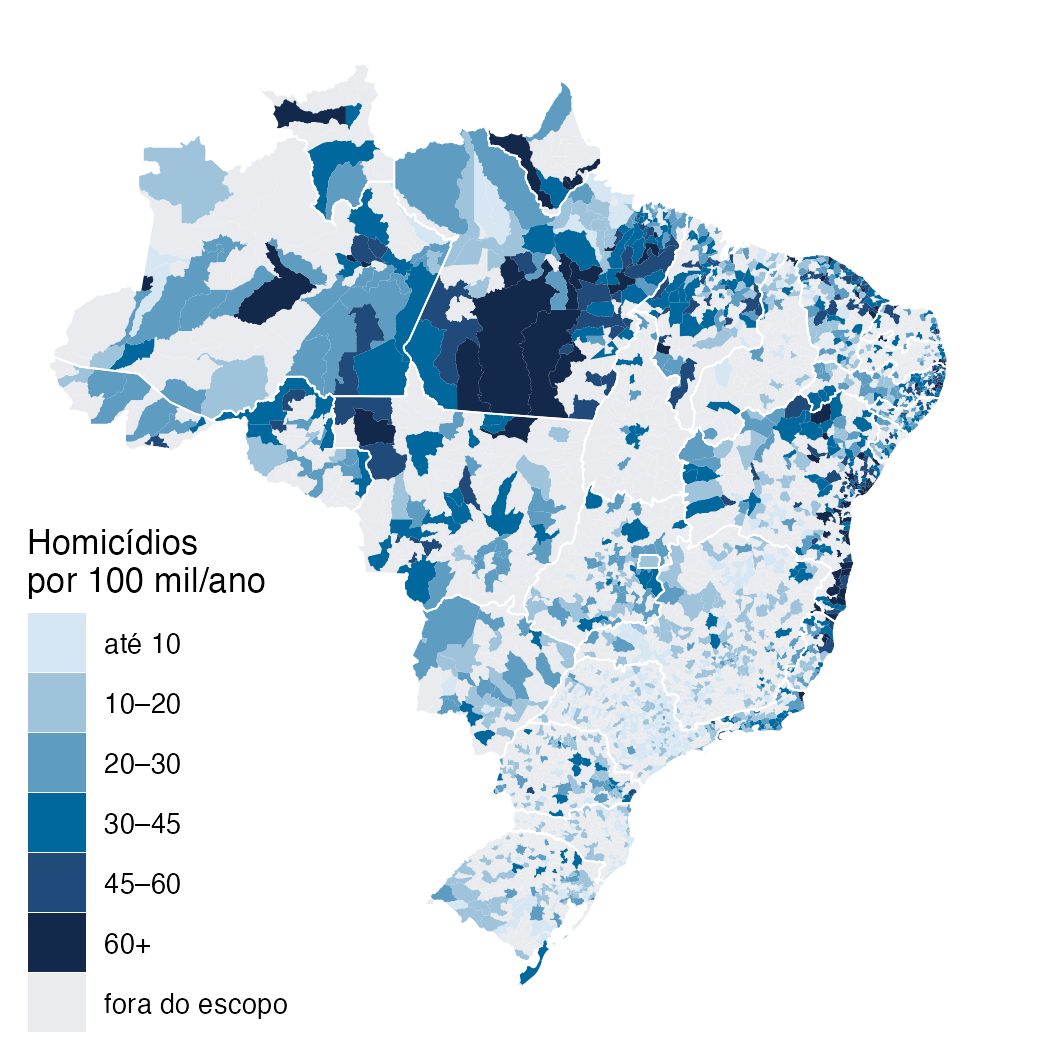
\includegraphics[width=\linewidth,height=0.7\textheight,keepaspectratio]{e2_mapa_taxa.png}
\fonte{SIM/DATASUS; IBGE (malha municipal 2022). Em cinza: fora do escopo.}
\column{0.62\textwidth}
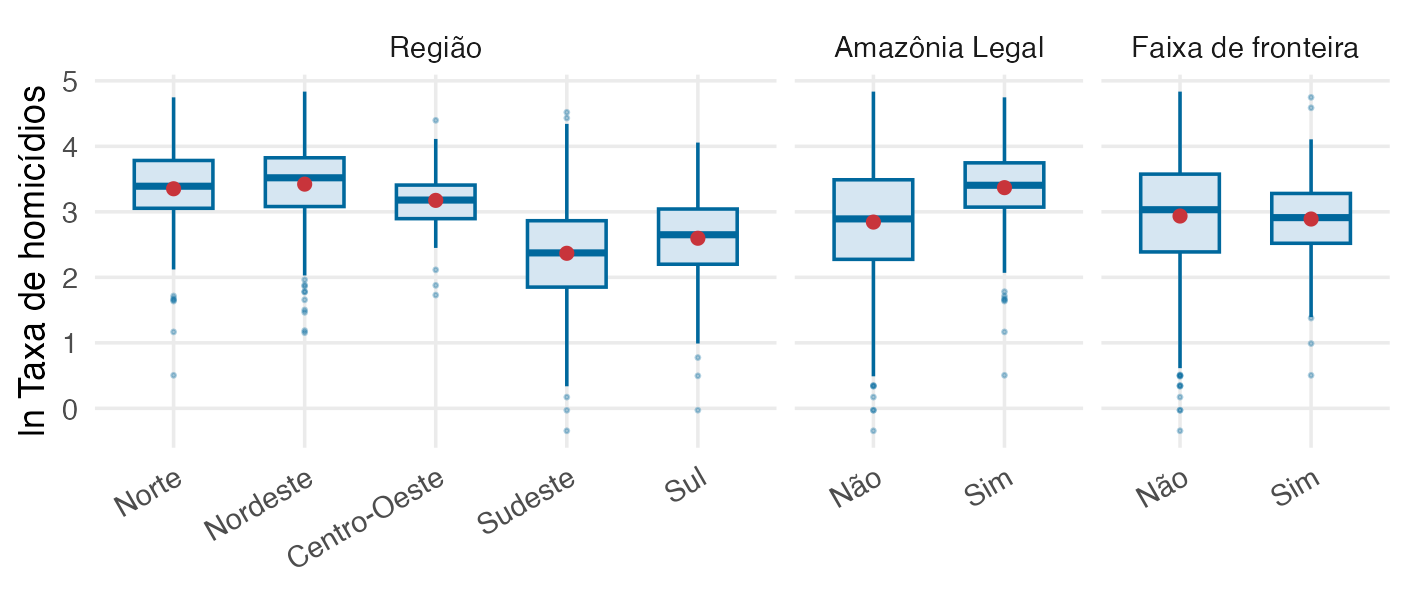
\includegraphics[width=\linewidth,keepaspectratio]{e3_box_regiao.png}
\fonte{Ponto vermelho: média. Elaboração própria.}
\vspace{0.3em}
\begin{itemize}\footnotesize
\item Norte e Nordeste acima de Sudeste e Sul
\item Mediana na Amazônia Legal: \nMedAma, contra \nMedForaAma; na faixa de fronteira: \nMedFront, contra \nMedForaFront
\item No modelo: estado (UF) como variável categórica; a Amazônia Legal sai, redundante com a UF
\end{itemize}
\end{columns}
\end{frame}

% -----------------------------------------------------------------------------
\begin{frame}{Correlação linear com ln(taxa)}
\begin{columns}[c]
\column{0.6\textwidth}
\fig{e5_correlacao.png}
\fonte{SIM/DATASUS; IBGE; INEP. Coeficiente de Pearson. Elaboração própria.}
\column{0.38\textwidth}
\begin{itemize}\small
\item Maior $|r|$: \nCorMaxVar{} (\nCorMax)
\item Nenhuma variável isolada basta: modelo múltiplo
\end{itemize}
\end{columns}
\end{frame}

% -----------------------------------------------------------------------------
\begin{frame}{Correlação entre as explicativas}
\begin{columns}[c]
\column{0.6\textwidth}
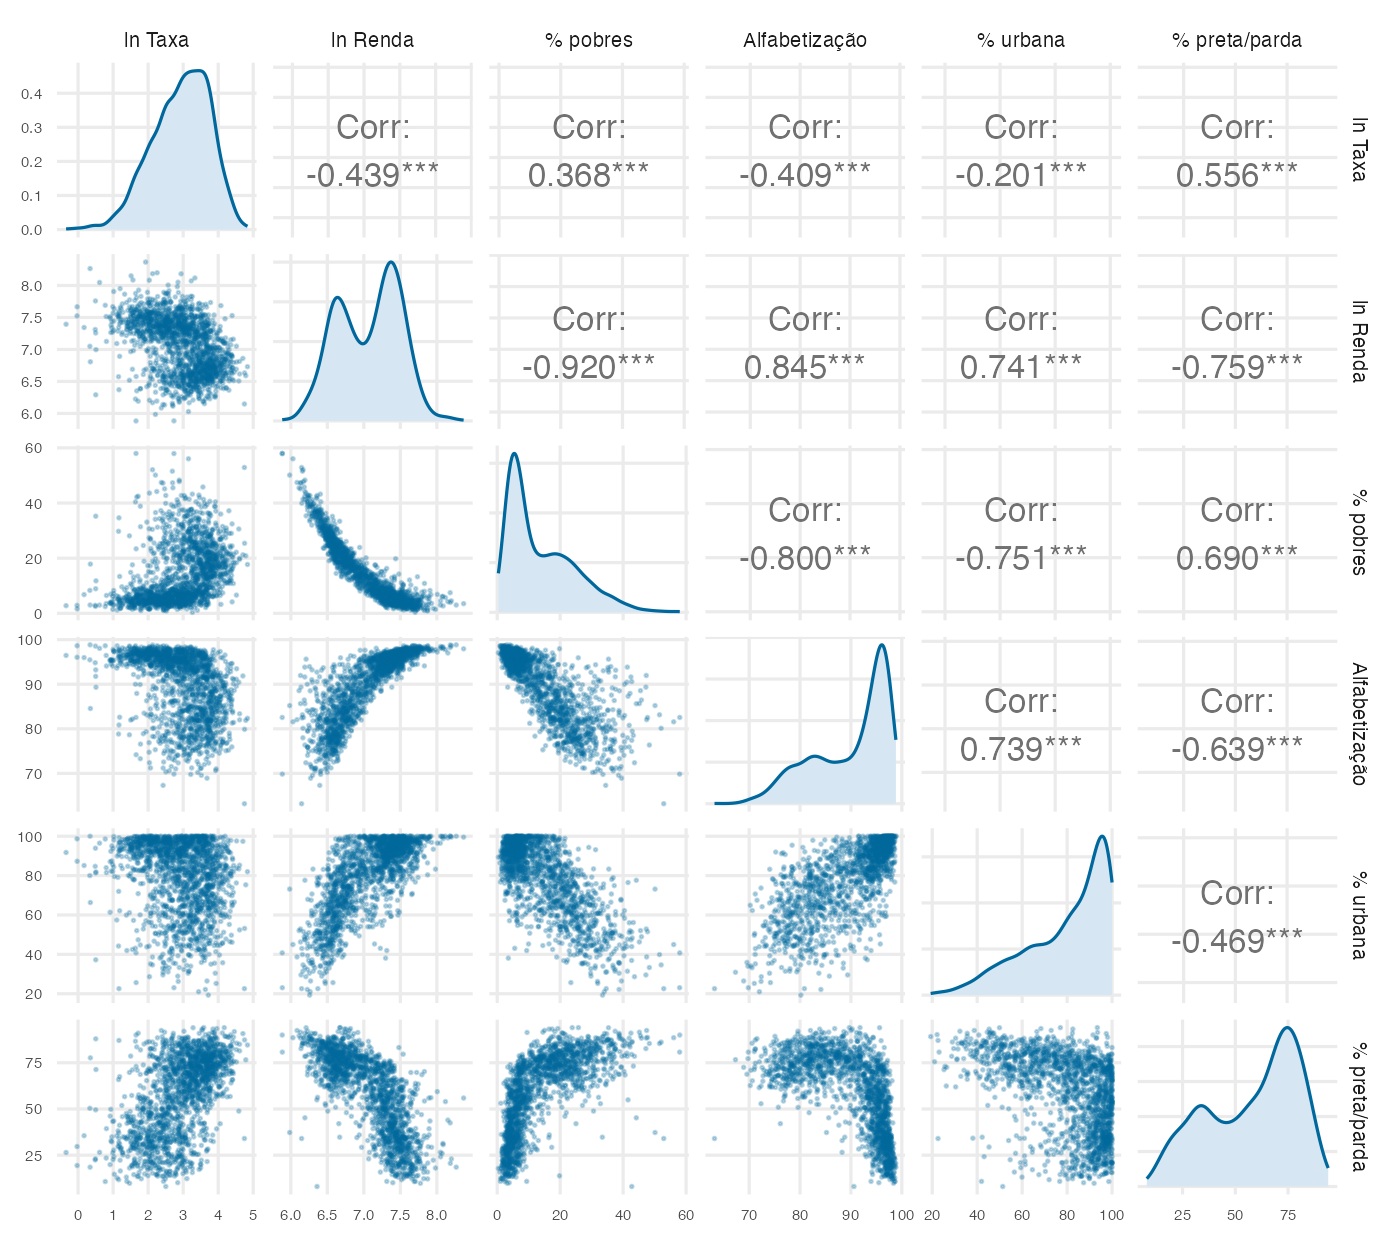
\includegraphics[width=\linewidth,height=0.84\textheight,keepaspectratio]{e8_pares.png}
\fonte{SIM/DATASUS; IBGE. Elaboração própria.}
\column{0.38\textwidth}
\begin{itemize}\small
\item Renda, \% pobres e alfabetização: $|r|$ até \nCorTrio{} entre si
\item As três medem quase o mesmo: VIF da renda \nVIFrenda{} com as três no modelo
\item No modelo fica só a renda; \% pobres e alfabetização saem
\end{itemize}
\end{columns}
\end{frame}

% -----------------------------------------------------------------------------
\begin{frame}{Relação não linear com a renda}
\begin{columns}[c]
\column{0.6\textwidth}
\fig{e7_box_renda.png}
\fonte{SIM/DATASUS; IBGE. Décimos de renda per capita. Elaboração própria.}
\column{0.38\textwidth}
\begin{itemize}\small
\item Taxa maior nos décimos intermediários (pico perto de R\$ \nRendaDecilPico)
\item Forma de U invertido
\item No modelo: polinômio de 2ª ordem na renda
\end{itemize}
\end{columns}
\end{frame}

% -----------------------------------------------------------------------------
\section[Modelo]{Ajuste preliminar do modelo}
\begin{frame}{Transformação da resposta (Box-Cox)}
\begin{columns}[c]
\column{0.6\textwidth}
\fig{m1_boxcox.png}
\fonte{Elaboração própria; modelo com todas as explicativas e a UF.}
\column{0.38\textwidth}
\begin{itemize}\small
\item Box e Cox (1964): $\hat\lambda = \nLambda$; IC 95\%: [\nLambdaInf; \nLambdaSup]
\item Adotado $\lambda = 0$ ($\ln Y$), por interpretabilidade (efeitos lidos em \%), embora fique fora do IC
\item Shapiro-Wilk: $W$ de \nSWy{} ($Y$) para \nSWln{} ($\ln Y$)
\end{itemize}
\end{columns}
\end{frame}

% -----------------------------------------------------------------------------
\begin{frame}{Especificação do modelo}
\[
\ln Y_i = \beta_0 + \beta_1 r_i + \beta_2 r_i^2 + \mathbf{x}_i^{\top}\bm{\delta} + \sum_{k=1}^{\nNumUF} \gamma_k D_{ik} + \varepsilon_i,
\qquad \varepsilon_i \overset{\text{iid}}{\sim} N(0, \sigma^2)
\]
\begin{itemize}\small
\setlength{\itemsep}{0.3em}
\item $r_i$: ln da renda per capita, centrada na média (reduz a correlação entre $r$ e $r^2$ de \nCorQuadSem{} para \nCorQuadCen)
\item $\mathbf{x}_i$: as demais \nNumX{} explicativas dos blocos A a D
\item $D_{ik}$: indicadora da UF $k$ (referência: SP)
\item Mínimos quadrados ordinários; $n = \nMunEsc$ municípios e \nNumPar{} parâmetros
\end{itemize}
\end{frame}

% -----------------------------------------------------------------------------
\begin{frame}{Construção do modelo em blocos}
\begin{columns}[c]
\column{0.58\textwidth}
\footnotesize
\renewcommand{\arraystretch}{1.3}
\setlength{\tabcolsep}{4pt}
\begin{tabular}{@{}lrr@{}}
\toprule
\textbf{Bloco} & \textbf{$F$ parcial} & \textbf{$R^2_a$}\\
\midrule
A: renda e desigualdade & --- & 0,28\\
B: + demografia & 71,8 & 0,35\\
C: + fronteira e registro & 101,5 & 0,39\\
D: + educação e migração & 46,9 & 0,44\\
\rowcolor{fundo}\textbf{E: + estado} & \textbf{24,8} & \textbf{0,59}\\
\bottomrule
\end{tabular}

\fonte{Elaboração própria. $F$ parcial pelas somas de quadrados extras.}
\column{0.40\textwidth}
\begin{itemize}\small
\item $H_0$: os coeficientes do bloco são nulos; rejeitada em todos os blocos
\item Maior ganho de $R^2_a$ com o estado (bloco E)
\item UF além da região: $F = \nFuf$ (\nGlUF{} gl), $p$ \nPUF; $R^2_a$ de \nRdoisAregiao{} para \nRdoisA
\end{itemize}
\end{columns}
\end{frame}

% -----------------------------------------------------------------------------
\begin{frame}{Estimativas: efeito de cada variável na taxa}
\begin{columns}[c]
\column{0.74\textwidth}
\scriptsize
\renewcommand{\arraystretch}{1.12}
\setlength{\tabcolsep}{2.5pt}
\begin{tabular}{@{}cllrcr@{}}
\toprule
\textbf{Hip.} & \textbf{Variável} & \textbf{Mudança} & \textbf{Taxa} & \textbf{IC 95\%} & \textbf{$p$}\\
\midrule
 & Renda & --- & U invertido & --- & $<$0,001\\
 & \% preta ou parda & +10 pontos & $+$19,6\% & [$+$15,8; $+$23,6] & $<$0,001\\
 & \% urbana & +10 pontos & $+$9,4\% & [$+$6,5; $+$12,3] & $<$0,001\\
H2 & Distorção idade-série (EM) & +10 pontos & $+$6,1\% & [$+$1,5; $+$10,9] & 0,009\\
H2 & Frequência escolar 15–17 & +5 pontos & $-$5,7\% & [$-$8,3; $-$3,1] & $<$0,001\\
H2 & Abandono no ensino médio & +5 pontos & $+$4,3\% & [$+$0,6; $+$8,2] & 0,022\\
H1 & Desigualdade & +0,1 & $+$3,2\% & [$+$0,7; $+$5,9] & 0,013\\
H3 & Migração recente & +5 pontos & $+$3,0\% & [$+$0,6; $+$5,5] & 0,014\\
 & Desocupação & +1 ponto & $-$1,4\% & [$-$2,5; $-$0,2] & 0,024\\
 & \% intenção indeterminada & +1 ponto & $-$1,2\% & [$-$1,5; $-$0,8] & $<$0,001\\
\bottomrule
\end{tabular}

\fonte{Elaboração própria. Efeito $= 100\,[\exp(b\,\Delta) - 1]\%$, demais variáveis constantes.}
\column{0.24\textwidth}
\begin{itemize}\footnotesize
\item Sinais consistentes com H1, H2 e H3
\item $R^2 = \nRdoisE$; $R^2_a = \nRdoisA$
\item $F = \nFglobal$ (\nGlUm{} e \nGlDois{} gl); $p$ \nFglobalP
\item \textcolor{gray}{Não significativas (5\%): \nNaoSig}
\end{itemize}
\end{columns}
\end{frame}

% -----------------------------------------------------------------------------
\begin{frame}{Efeito da renda previsto pelo modelo}
\begin{columns}[c]
\column{0.6\textwidth}
\fig{m7_efeito_renda.png}
\fonte{Elaboração própria. Demais variáveis na média; UF = SP. Faixa: IC 95\% da resposta esperada.}
\column{0.38\textwidth}
\begin{itemize}\small
\item $\hat\beta_2$ = \nBetaDois{} ($p$ \nBetaDoisP): concavidade
\item Máximo em $r^{*} = -\hat\beta_1 / (2\hat\beta_2)$: renda de \alert{R\$ \nPico}
\item Taxa esperada menor nos extremos de renda
\end{itemize}
\end{columns}
\end{frame}

% -----------------------------------------------------------------------------
\begin{frame}{Diagnóstico dos resíduos}
\begin{columns}[c]
\column{0.31\textwidth}
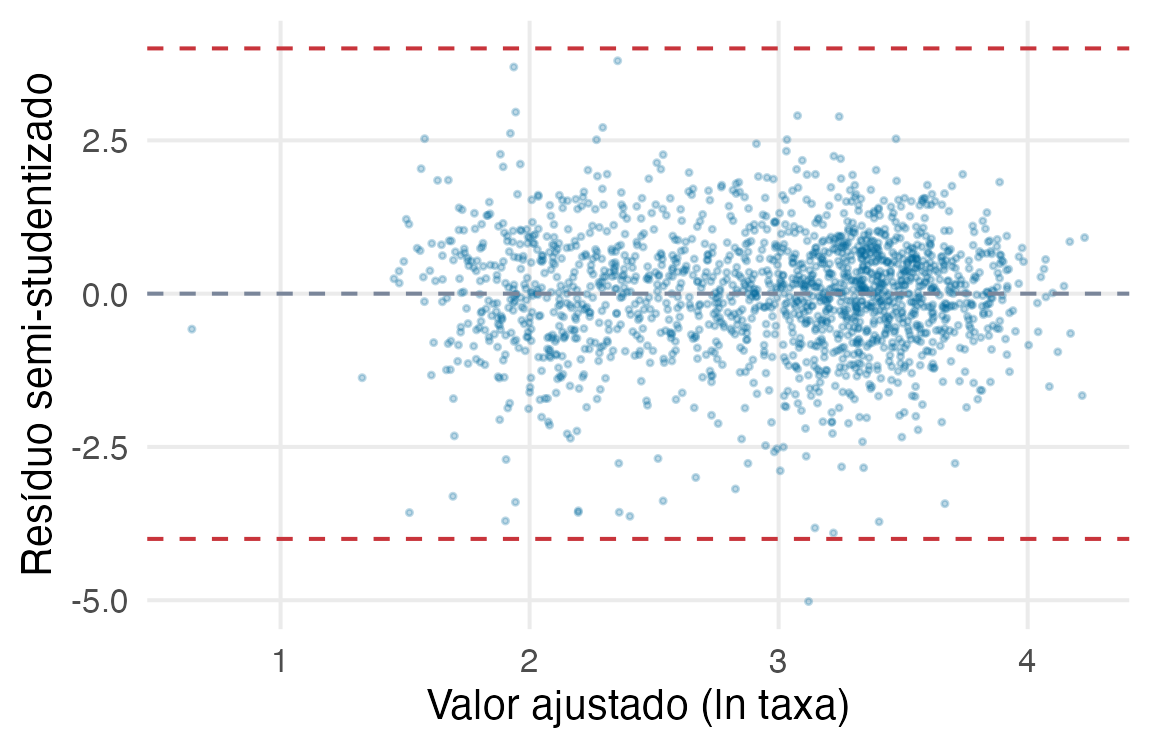
\includegraphics[width=\linewidth,height=0.55\textheight,keepaspectratio]{m3a_residuos_ajustados.png}
\fonte{Elaboração própria. Resíduos semi-studentizados.}
\column{0.67\textwidth}
\scriptsize
\renewcommand{\arraystretch}{1.25}
\setlength{\tabcolsep}{3pt}
\begin{tabular}{@{}llrr@{}}
\toprule
\textbf{Pressuposto} & \textbf{Teste} & \textbf{Estatística} & \textbf{$p$}\\
\midrule
Normalidade & Shapiro-Wilk & $W = \nSW$ & \nSWp\\
Homocedasticidade & Breusch-Pagan & \nBP{} (\nBPgl{} gl) & \nBPp\\
Independência & Durbin-Watson & $d = \nDW$ & \nDWp\\
Multicolinearidade & VIF máximo & \nVIFrendaFinal{} (renda) & ---\\
Outliers & $|e^{*}_i| \geq 4$ & \nNout & ---\\
\bottomrule
\end{tabular}
\par\vspace{0.1em}{\tiny\color{black!60}VIF das demais variáveis $\leq$ \nVIFdemaisMax. Outlier: \nOutNomes.}
\vspace{0.3em}

\begin{itemize}\scriptsize
\item Breusch-Pagan rejeita $H_0$: erros-padrão e valores $p$ são aproximados
\item Shapiro-Wilk rejeita com $W$ próximo de 1 ($n$ grande); cauda esquerda mais pesada que a normal
\item Durbin-Watson na ordem do código IBGE (quase alfabética dentro da UF): não avalia a dependência entre vizinhos geográficos
\end{itemize}
\end{columns}
\end{frame}

% -----------------------------------------------------------------------------
\section[Conclusão]{Considerações e próximos passos}
\begin{frame}{Considerações e próximos passos}
\begin{columns}[T]
\column{0.49\textwidth}
\textbf{\color{navy}Resposta preliminar à pergunta}
\begin{itemize}\small
\item Mais homicídios com mais desigualdade (H1), exclusão escolar (H2) e migração recente (H3)
\item Renda em U invertido: pico em R\$ \nPico
\item Também mais homicídios com mais \% preta ou parda e urbanização
\item Grande diferença entre estados
\end{itemize}
\column{0.49\textwidth}
\textbf{\color{navy}Em relação à literatura}
\begin{itemize}\small
\item Urbanização e desigualdade: mesmo sinal de Wanzinack et al. (2022)
\item Diferença entre estados: como em Castellucci e Silva (2026)
\end{itemize}
\vspace{0.3em}
\textbf{\color{navy}Próximos passos}
\begin{itemize}\small
\item Seleção de variáveis: $C_p$, AIC, BIC e PRESS
\item Variância não constante
\item Correlação dos resíduos entre vizinhos, como em Barros et al. (2020)
\end{itemize}
\end{columns}
\end{frame}

\begin{frame}[plain,c,standout]
\centering
{\Huge\color{navy}Obrigado!}\par
\vspace{1em}
{\large Perguntas?}
\end{frame}

% -----------------------------------------------------------------------------
\appendix

\begin{frame}{Apêndice A · Coeficientes estimados}
\scriptsize
\renewcommand{\arraystretch}{1.1}
\begin{tabular*}{\textwidth}{@{\extracolsep{\fill}}lrrrlrrr@{}}
\toprule
\textbf{Termo} & \textbf{$b$} & \textbf{EP} & \textbf{$p$} & \textbf{Termo} & \textbf{$b$} & \textbf{EP} & \textbf{$p$}\\
\midrule
ln renda (centr.) & $-$0,106 & 0,105 & 0,310 & \% homens 15--29 & $-$0,024 & 0,017 & 0,158\\
ln renda² & $-$0,548 & 0,085 & $<$0,001 & Fronteira & $-$0,077 & 0,060 & 0,200\\
Desigualdade & 0,319 & 0,129 & 0,013 & \% indeterminada & $-$0,012 & 0,002 & $<$0,001\\
Desocupação & $-$0,014 & 0,006 & 0,024 & Freq. escolar 15--17 & $-$0,012 & 0,003 & $<$0,001\\
\% urbana & 0,009 & 0,001 & $<$0,001 & Abandono EM & 0,008 & 0,004 & 0,022\\
ln densidade & 0,013 & 0,012 & 0,273 & Distorção EM & 0,006 & 0,002 & 0,009\\
\% preta ou parda & 0,018 & 0,002 & $<$0,001 & Migração recente & 0,006 & 0,002 & 0,014\\
\bottomrule
\end{tabular*}

\vspace{0.5em}

Resposta $\ln Y$; MQO; $n = \nMunEsc$. Mais \nNumUF{} indicadoras de UF (referência: SP), omitidas.
$\hat\sigma = \nSigma$; $R^2 = \nRdoisE$; $R^2_a = \nRdoisA$. EP: erro-padrão.
\end{frame}

\begin{frame}{Apêndice B · Referências}
\tiny
\begin{columns}[T]
\column{0.49\textwidth}\setlength{\parskip}{0.5em}
ARANSIOLA, T. J.; CECCATO, V.; JUSTUS, M. Growth of lethal violence in Brazil 2000--2017: a space-temporal analysis of homicides. \textit{Journal of Contemporary Criminal Justice}, 2022. DOI: 10.1177/10439862211034343.

BARROS, P. H. B.; BAGGIO, H. S.; BAGGIO, I. S. The socioeconomic determinants of crime in Brazil: the role of spatial spillovers and heterogeneity. \textit{Revista Brasileira de Segurança Pública}, v. 14, n. 2, p. 188--209, 2020.

BOX, G. E. P.; COX, D. R. An analysis of transformations. \textit{Journal of the Royal Statistical Society: Series B}, v. 26, n. 2, p. 211--252, 1964.

CASTELLUCCI, L. V.; SILVA, É. M. Fatores socioeconômicos da violência letal urbana em municípios brasileiros. \textit{E\&S Journal}, 2026.

FAJNZYLBER, P.; LEDERMAN, D.; LOAYZA, N. Inequality and violent crime. \textit{Journal of Law and Economics}, v. 45, n. 1, p. 1--39, 2002.

FERRARI, D. \textit{GED-16: Análise de Regressão} (apostila). São José dos Campos: ITA. Disponível em: \texttt{www.ief.ita.br/\~{}denise/GED16/Apostila/}.

IBGE. \textit{Censo Demográfico 2022}. Rio de Janeiro: IBGE. Sistema IBGE de Recuperação Automática (SIDRA).
\column{0.49\textwidth}\setlength{\parskip}{0.5em}
INEP. \textit{Indicadores Educacionais 2022}: taxas de rendimento e distorção idade-série por município. Brasília: INEP.

LOCHNER, L.; MORETTI, E. The effect of education on crime: evidence from prison inmates, arrests, and self-reports. \textit{American Economic Review}, v. 94, n. 1, p. 155--189, 2004.

MINISTÉRIO DA SAÚDE. \textit{Sistema de Informações sobre Mortalidade (SIM)}. DATASUS, TabNet.

MURRAY, J.; CERQUEIRA, D. R. C.; KAHN, T. Crime and violence in Brazil: systematic review of time trends, prevalence rates and risk factors. \textit{Aggression and Violent Behavior}, v. 18, n. 5, p. 471--483, 2013.

SAMPSON, R. J.; GROVES, W. B. Community structure and crime: testing social-disorganization theory. \textit{American Journal of Sociology}, v. 94, n. 4, p. 774--802, 1989.

UNODC. \textit{Global Study on Homicide 2023}. Viena: United Nations Office on Drugs and Crime, 2023.

WANZINACK, C.; SIGNORELLI, M. C.; REIS, C. Violence and social determinants of health in Brazil: association between homicides, urbanization, population, inequality, and development. \textit{Cadernos de Saúde Pública}, v. 38, n. 10, e00282621, 2022.
\end{columns}
\end{frame}

\end{document}
